\newpage

\pagenumbering{arabic}

\setcounter{page}{1}

\section{迁移学习基本概念} \label{overview}%------------------------------

\subsection{引子}

冬末春初,北京的天气渐渐暖了起来。这是一句再平常不过的气候描述。对于我们在北半球生活的人来说,这似乎是一个司空见惯的现象。北京如此,纽约如此,东京如此,巴黎也如此。然而此刻,假如我问你,阿根廷的首都布宜诺斯艾利斯,天气如何?稍稍有点地理常识的人就该知道,阿根廷位于南半球,天气恰恰相反:正是夏末秋初的时候,天气渐渐凉了起来。

我们何以根据北京的天气来推测出纽约、东京和巴黎的天气?我们又何以不能用相同的方式来推测阿根廷的天气?

答案显而易见:因为它们的地理位置不同。除去阿根廷在南半球之外,其他几个城市均位于北半球,故而天气变化相似。

我们可以利用这些地点\textit{地理位置的相似性和差异性},很容易地推测出其他地点的天气。这样一个简单的事实,就引出了我们要介绍的主题:\textit{迁移学习}。

\subsection{迁移学习的概念}

迁移学习,顾名思义,就是要进行迁移。放到我们人工智能和机器学习的学科里讲,迁移学习是一种学习的思想和模式。

我们都对机器学习有了基本的了解。机器学习是人工智能的一大类重要方法,也是目前发展最迅速、效果最显著的方法。机器学习解决的是让机器自主地从数据中获取知识,从而应用于新的问题中。迁移学习作为机器学习的一个重要分支,侧重于将已经学习过的知识迁移应用于新的问题中。

迁移学习的核心问题是,找到新问题和原问题之间的相似性,才可以顺利地实现知识的迁移。比如在我们一开始说的天气问题中,那些北半球的天气之所以相似,是因为它们的地理位置相似;而南北半球的天气之所以有差异,也是因为地理位置有根本不同。

其实我们人类对于迁移学习这种能力,是与生俱来的。比如,我们如果已经会打乒乓球,就可以类比着学习打网球。再比如,我们如果已经会下中国象棋,就可以类比着下国际象棋。因为这些活动之间,往往有着极高的相似性。生活中常用的“\textit{举一反三}”、“\textit{照猫画虎}”就很好地体现了迁移学习的思想。

回到我们的问题中来。我们用更加学术更加机器学习的语言来对迁移学习下一个定义。迁移学习,是指利用数据、任务、或模型之间的相似性,将在旧领域学习过的模型,应用于新领域的一种学习过程。

迁移学习最权威的综述文章是香港科技大学杨强教授团队的A survey on transfer learning~\cite{pan2010survey}。

图~\ref{fig-transfer}简要表示了一个迁移学习过程。图~\ref{fig-example}给出了生活中常见的迁移学习的例子。

\begin{figure}[htbp]
	\centering
	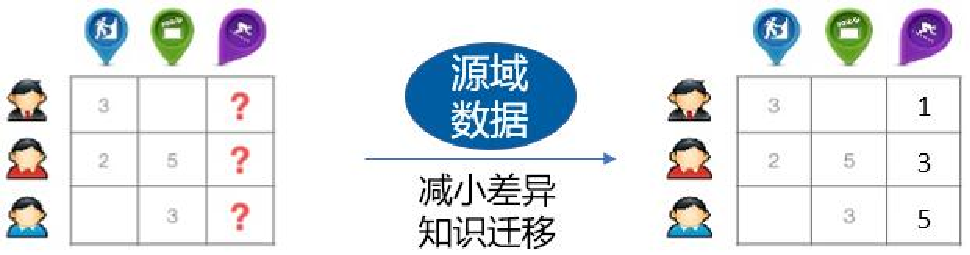
\includegraphics[scale=0.5]{./figures/fig-introduction-transfer.pdf}
	\caption{迁移学习示意图}
	\label{fig-transfer}
\end{figure}

\begin{figure}[htbp]
	\centering
	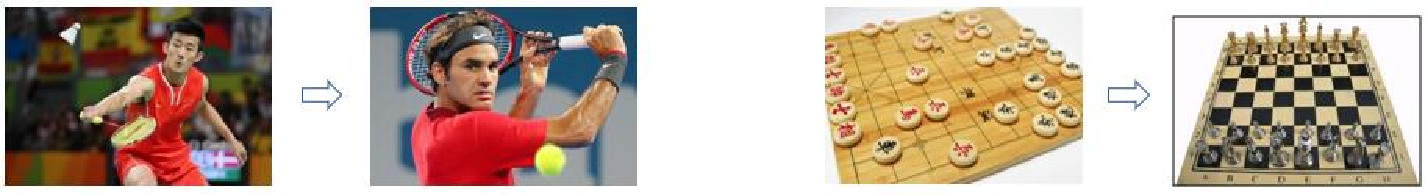
\includegraphics[scale=0.5]{./figures/fig-introduction-example.pdf}
	\caption{迁移学习的例子}
	\label{fig-example}
\end{figure}

值得一提的是,新华社报道指出,迁移学习是中国领先于世界的少数几个人工智能领域之一~\cite{xinhua}。中国的人工智能赶超的机会来了!


\subsection{为什么需要迁移学习?}

了解了迁移学习的概念之后,紧接着还有一个非常重要的问题:迁移学习的目的是什么? 或者说,\textit{为什么要用迁移学习}?

我们把原因概括为以下四个方面:

\textbf{1. 大数据与少标注之间的矛盾。}

\begin{figure}[htbp]
	\centering
	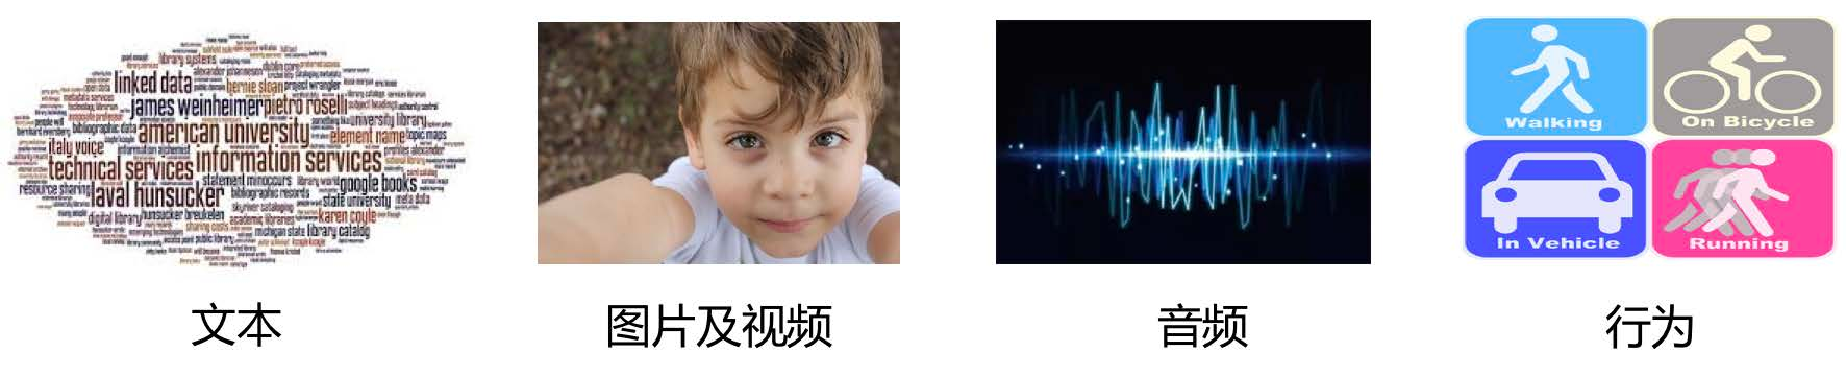
\includegraphics[scale=0.42]{./figures/fig-introduction-data.pdf}
	\caption{多种多样的数据来源}
	\label{fig-introduction-data}
\end{figure}

我们正处在一个大数据时代,每天每时,社交网络、智能交通、视频监控、行业物流等,都产生着海量的图像、文本、语音等各类数据。数据的增多,使得机器学习和深度学习模型可以依赖于如此\textit{海量的数据},持续不段地训练和更新相应的模型,使得模型的性能越来越好,越来越适合特定场景的应用。然而,这些大数据带来了严重的问题:总是缺乏完善的\textit{数据标注}。

众所周知,机器学习模型的训练和更新,均依赖于数据的标注。然而,尽管我们可以获取到海量的数据,这些数据往往是很初级的原始形态,很少有数据被加以正确的人工标注。数据的标注是一个耗时且昂贵的操作,目前为止,尚未有行之有效的方式来解决这一问题。这给机器学习和深度学习的模型训练和更新带来了挑战。反过来说,特定的领域,因为没有足够的标定数据用来学习,使得这些领域一直不能很好的发展。

\textbf{2. 大数据与弱计算之间的矛盾。}

大数据,就需要大设备、强计算能力的设备来进行存储和计算。然而,大数据的大计算能力,是"有钱人"才能玩得起的游戏。比如Google,Facebook,Microsoft,这些巨无霸公司有着雄厚的计算能力去利用这些数据训练模型。例如,ResNet需要很长的时间进行训练。Google TPU也都是有钱人的才可以用得起的。

绝大多数普通用户是不可能具有这些强计算能力的。这就引发了大数据和弱计算之间的矛盾。在这种情况下,普通人想要利用这些海量的大数据去训练模型完成自己的任务,基本上不太可能。那么如何让普通人也能利用这些数据和模型?

\begin{figure}[htbp]
	\centering
	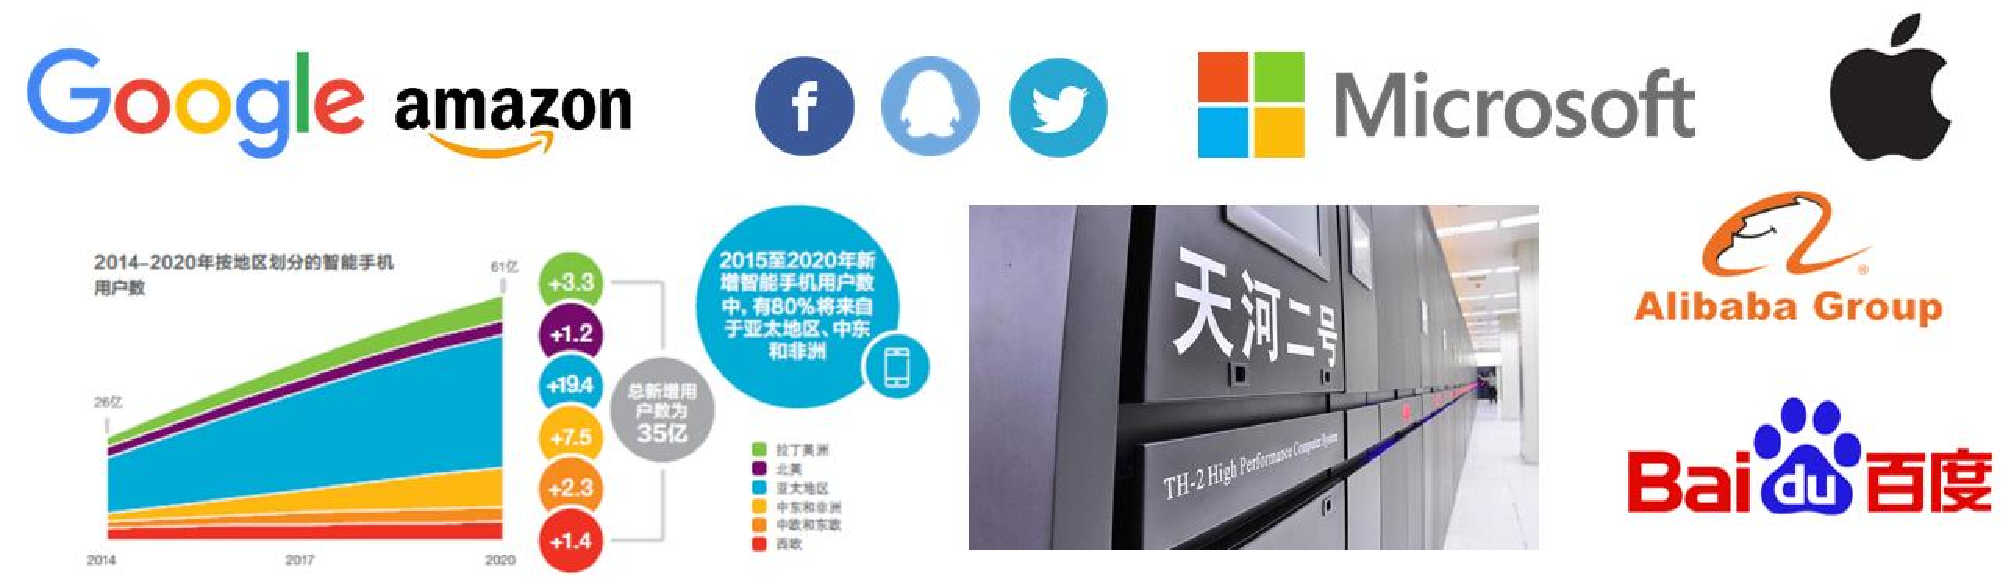
\includegraphics[scale=0.42]{./figures/fig-introduction-bigdata.pdf}
	\caption{大数据与强计算能力}
	\label{fig-bigdata}
\end{figure}

\textbf{3. 普适化模型与个性化需求之间的矛盾。}

机器学习的目标是构建一个尽可能通用的模型,使得这个模型对于不同用户、不同设备、不同环境、不同需求,都可以很好地进行满足。这是我们的美好愿景。这就是要尽可能地提高机器学习模型的\textit{泛化能力},使之适应不同的数据情形。基于这样的愿望,我们构建了多种多样的普适化模型,来服务于现实应用。然而,这只能是我们竭尽全力想要做的,目前却始终无法彻底解决的问题。人们的个性化需求五花八门,短期内根本无法用一个通用的模型去满足。比如导航模型,可以定位及导航所有的路线。但是不同的人有不同的需求。比如有的人喜欢走高速,有的人喜欢走偏僻小路,这就是个性化需求。并且,不同的用户,通常都有不同的\textit{隐私需求}。这也是构建应用需要着重考虑的。

所以目前的情况是,我们对于每一个通用的任务都构建了一个通用的模型。这个模型可以解决绝大多数的公共问题。但是具体到每个个体、每个需求,都存在其唯一性和特异性,一个普适化的通用模型根本无法满足。那么,能否将这个通用的模型加以改造和适配,使其更好地服务于人们的个性化需求?

\begin{figure}[htbp]
	\centering
	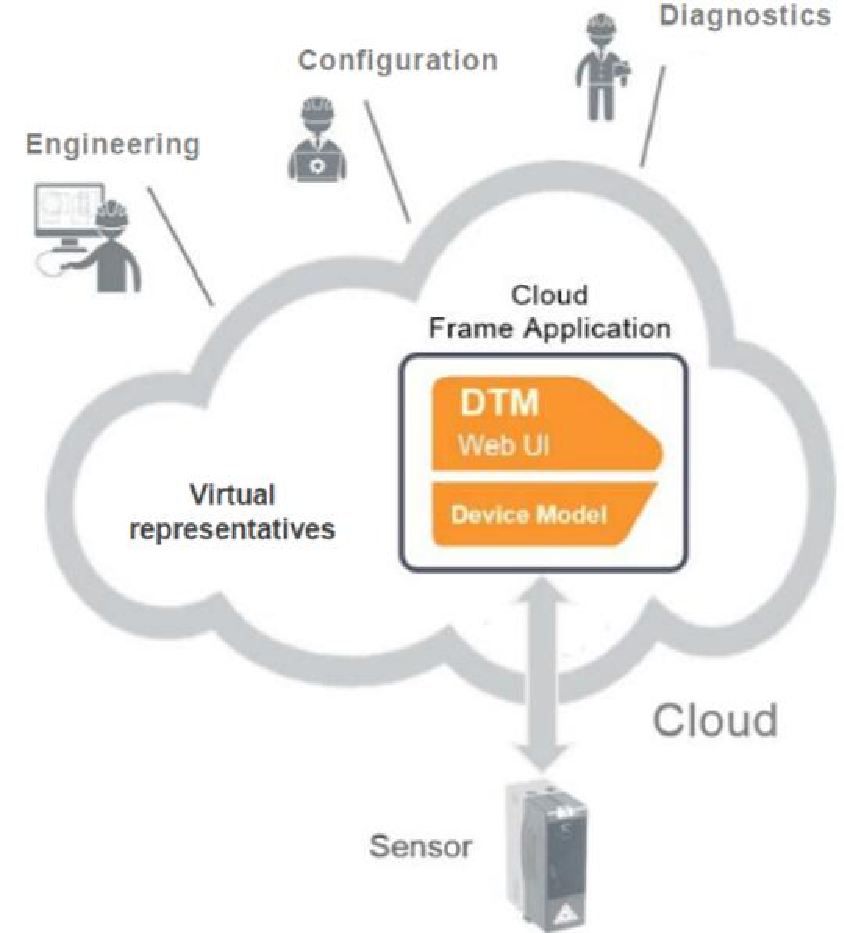
\includegraphics[scale=0.45]{./figures/fig-introduction-model.pdf}
	\caption{普适化模型与个性化需求}
	\label{fig-privacy}
\end{figure}

\textbf{4. 特定应用的需求。}

机器学习已经被广泛应用于现实生活中。在这些应用中,也存在着一些特定的应用,它们面临着一些现实存在的问题。比如推荐系统的\textit{冷启动}问题。一个新的推荐系统,没有足够的用户数据,如何进行精准的推荐? 一个崭新的图片标注系统,没有足够的标签,如何进行精准的服务?现实世界中的应用驱动着我们去开发更加便捷更加高效的机器学习方法来加以解决。

\begin{figure}[htbp]
	\centering
	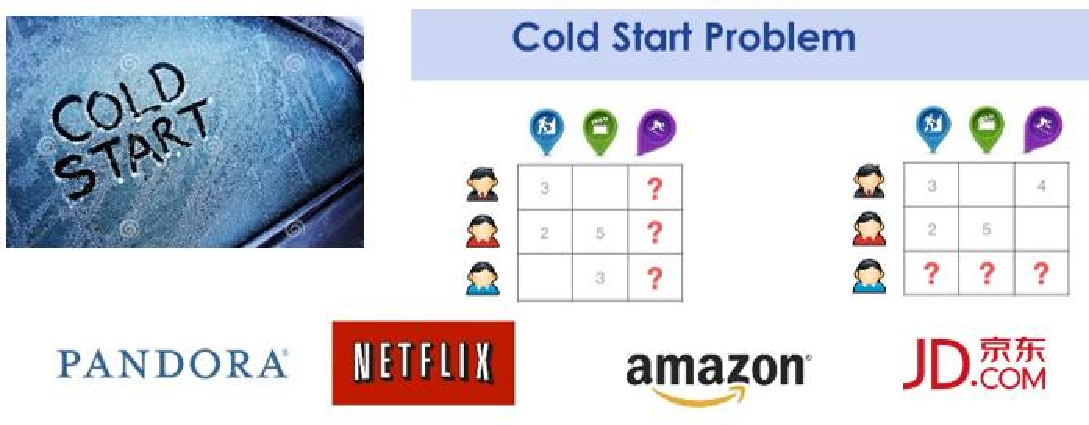
\includegraphics[scale=0.45]{./figures/fig-introduction-coldstart.pdf}
	\caption{特定应用需求:冷启动}
	\label{fig-coldstart}
\end{figure}

上述存在的几个重要问题,使得传统的机器学习方法疲于应对。迁移学习则可以很好地进行解决。那么,\textbf{迁移学习是如何进行解决的呢?}

1. 大数据与少标注:迁移数据标注

单纯地凭借少量的标注数据,无法准确地训练高可用度的模型。为了解决这个问题,我们直观的想法是:多增加一些标注数据不就行了?但是不依赖于人工,如何增加标注数据?

利用迁移学习的思想,我们可以寻找一些与目标数据相近的有标注的数据,从而利用这些数据来构建模型,增加我们目标数据的标注。

2. 大数据与弱计算:模型迁移

不可能所有人都有能力利用大数据快速进行模型的训练。利用迁移学习的思想,我们可以将那些大公司在大数据上训练好的模型,迁移到我们的任务中。针对于我们的任务进行微调,从而我们也可以拥有在大数据上训练好的模型。更进一步,我们可以将这些模型针对我们的任务进行自适应更新,从而取得更好的效果。

3. 普适化模型与个性化需求:自适应学习

为了解决个性化需求的挑战,我们利用迁移学习的思想,进行自适应的学习。考虑到不同用户之间的相似性和差异性,我们对普适化模型进行灵活的调整,以便完成我们的任务。

4. 特定应用的需求:相似领域知识迁移

为了满足特定领域应用的需求,我们可以利用上述介绍过的手段,从数据和模型方法上进行迁移学习。

表\ref{tb-whytransfer}概括地描述了迁移学习的必要性。

\begin{table}[htbp]
	\centering
	\caption{迁移学习的必要性}
	\label{tb-whytransfer}
	\begin{tabular}{|c|c|c|}
		\hline
		\textbf{矛盾} & \textbf{传统机器学习} & \textbf{迁移学习} \\ \hline
		大数据与少标注 & 增加人工标注,但是昂贵且耗时 & 数据的迁移标注 \\ \hline
		大数据与弱计算 & 只能依赖强大计算能力,但是受众少 & 模型迁移 \\ \hline
		普适化模型与个性化需求 & 通用模型无法满足个性化需求 & 模型自适应调整 \\ \hline
		特定应用 & 冷启动问题无法解决 & 数据迁移 \\ \hline
	\end{tabular}
\end{table}

\subsection{与已有概念的区别和联系}

迁移学习并不是一个横空出世的概念,它与许多已有的概念都有些联系,但是也有着一些区别。我们在这里汇总一些与迁移学习非常接近的概念,并简述迁移学习与它们的区别和联系。

\textbf{1. 迁移学习 VS 传统机器学习:}

迁移学习属于机器学习的一类,但它在如下几个方面有别于传统的机器学习(表~\ref{tb-introduction-machinelearning}):

\begin{table}[htbp]
\centering
\caption{传统机器学习与迁移学习的区别}
\label{tb-introduction-machinelearning}
\begin{tabular}{|l|l|l|}
\hline
\multicolumn{1}{|c|}{\textbf{比较项目}} & \multicolumn{1}{c|}{\textbf{传统机器学习}} & \multicolumn{1}{c|}{\textbf{迁移学习}} \\ \hline
数据分布 & 训练和测试数据服从相同的分布 & 训练和测试数据服从不同的分布 \\ \hline
数据标注 & 需要足够的数据标注来训练模型 & 不需要足够的数据标注 \\ \hline
模型 & 每个任务分别建模 & 模型可以在不同任务之间迁移 \\ \hline
\end{tabular}
\end{table}

\textbf{2. 迁移学习 VS 终身学习:}

终身学习强调连续不断地在一个概念和任务上进行学习,模型持续优化。迁移学习则侧重于模型的迁移和共同学习。

\textbf{3. 迁移学习 VS 多任务学习:}

多任务学习指多个相关的任务一起协同学习;迁移学习则强调知识由一个领域迁移到另一个领域的过程。迁移是思想,多任务是其中的一个具体形式。

\textbf{4. 迁移学习 VS 领域自适应:}

领域自适应问题是迁移学习的研究内容之一,它侧重于解决特征空间一致、类别空间一致,仅特征分布不一致的问题。而迁移学习也可以解决上述内容不一致的情况。

\textbf{5. 迁移学习 VS 增量学习:}

增量学习侧重解决数据不断到来,模型不断更新的问题。迁移学习显然和其有着不同之处。

\textbf{6. 迁移学习 VS 自我学习:}

自我学习指的是模型不断地从自身处进行更新,而迁移学习强调知识在不同的领域间进行迁移。

\textbf{7. 迁移学习 VS 协方差漂移}

协方差漂移也是迁移学习要研究的问题之一,它特指数据的条件概率分布发生变化。

\subsection{负迁移}
我们都希望迁移学习能够比较顺利地进行,我们得到的结果也是满足我们要求的,皆大欢喜。然而,事情却并不总是那么顺利。这就引入了迁移学习中的一个负面现象,也就是所谓的\textbf{负迁移}。

用我们熟悉的成语来描述:如果说成功的迁移学习是“举一反三”、“照猫画虎”,那么负迁移则是“\textit{东施效颦}”。东施已经模仿西施捂着胸口皱着眉头,为什么她还是那么丑?

要理解负迁移,首先要理解什么是迁移学习。迁移学习指的是,利用数据和领域之间存在的相似性关系,把之前学习到的知识,应用于新的未知领域。迁移学习的核心问题是,找到两个领域的相似性。找到了这个相似性,就可以合理地利用,从而很好地完成迁移学习人物。比如,之前会骑自行车,要学习骑摩托车,这种相似性指的就是自行车和摩托车之间的相似性以及骑车体验的相似性。这种相似性在我们人类看来是可以接受的。

所以,如果这个相似性找的不合理,也就是说,\textit{两个领域之间不存在相似性,或者基本不相似},那么,就会大大损害迁移学习的效果。还是拿骑自行车来说,你要拿骑自行车的经验来学习开汽车,这显然是不太可能的。因为自行车和汽车之间基本不存在什么相似性。所以,这个任务基本上完不成。这时候,我们可以说出现了\textbf{负迁移(Negative Transfer)}。

所以,为什么东施和西施做了一样的动作,反而变得更丑了?\textit{因为东施和西施之间压根就不存在相似性。}

迁移学习领域权威学者、香港科技大学杨强教授发表的迁移学习的综述文章A survey on transfer learning~\cite{pan2010survey}给出了负迁移的一个定义:

\textit{负迁移指的是,在源域上学习到的知识,对于目标域上的学习产生负面作用。}

文章也引用了一些经典的解决负迁移问题的文献。但是普遍较老,这里就不说了。

所以,产生负迁移的原因主要有:

\begin{itemize}
	\item 数据问题:源域和目标域压根不相似,谈何迁移?
	\item 方法问题:源域和目标域是相似的,但是,迁移学习方法不够好,没找到可迁移的成分。
\end{itemize}

负迁移给迁移学习的研究和应用带来了负面影响。在实际应用中,找到合理的相似性,并且选择或开发合理的迁移学习方法,能够避免负迁移现象。

\textbf{最新的研究成果}

随着研究的深入,已经有新的研究成果在逐渐克服负迁移的影响。杨强教授团队2015在数据挖掘领域顶级会议KDD上发表了传递迁移学习文章Transitive transfer learning~\cite{tan2015transitive},提出了传递迁移学习的思想。传统迁移学习就好比是\textit{踩着一块石头过河},传递迁移学习就好比是\textit{踩着连续的两块石头}。

更进一步,杨强教授团队在2017年人工智能领域顶级会议AAAI上发表了远领域迁移学习的文章Distant domain transfer learning~\cite{tan2017distant},可以用人脸来识别飞机!这就好比是\textit{踩着一连串石头过河}。这些研究的意义在于,传统迁移学习只有两个领域足够相似才可以完成,而当两个领域不相似时,传递迁移学习却可以利用处于这两个领域之间的若干领域,将知识传递式的完成迁移。这个是很有意义的工作,可以视为解决负迁移的有效思想和方法。可以预见在未来会有更多的应用前景。

图~\ref{fig-negative}对传递迁移学习给出了简明的示意。

\begin{figure}[htbp]
	\centering
	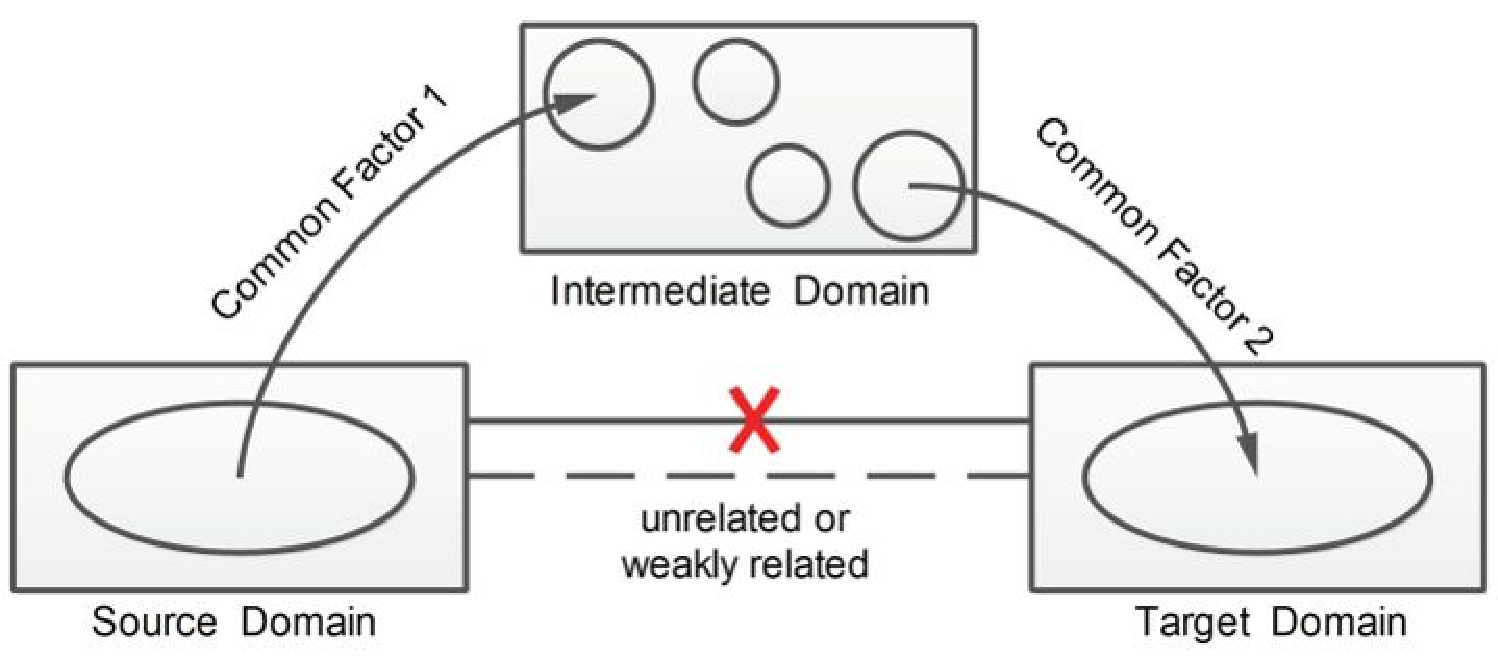
\includegraphics[scale=0.45]{./figures/fig-introduction-negativetransfer.pdf}
	\caption{传递式迁移学习示意图}
	\label{fig-negative}
\end{figure}

